%=====================================================================
% 3  Feynman 演算
% 原文：Section 3. Feynman calculus（arXiv:2409.03117v1, p. 28--38）
%=====================================================================
\section{Feynman 演算}

\begin{keytakeaways}
\begin{itemize}
  \item \textbf{物理图像：} 高斯测度下多项式期望值完全由两两缩并决定（Wick 定理）；含相互作用时，关联函数按 Feynman 图逐图求和，每条边携带传播子，每个顶点携带相互作用张量。
  \item \textbf{数学工具：} 配对计数（双阶乘）、图的自同构群与对称因子、生成函数取对数（连通图求和）、按普朗克常数的幂次作圈展开。
  \item \textbf{关键结论：} Feynman 定理把关联函数写成对全部图的求和，每项权重为普朗克常数的幂除以自同构群阶；对配分函数取对数后只剩连通图，且幂次等于圈数减一，最低阶即经典（树）近似。
  \item \textbf{易错点：} 对称因子不只来自顶点置换，交换多重边与翻转自环同样计入自同构；连通图取对数时，同构图不可区分的副本正是产生阶乘因子的来源。
\end{itemize}
\end{keytakeaways}

\bigskip
\noindent\rule{\textwidth}{0.6pt}
\bigskip

\subsection{Wick 定理}
设 $V$ 是 $d$ 维实向量空间，其体积元为 $dx$。
设 $S(x)$ 是紧区域 $D\subset V$ 上的光滑函数，边界光滑，且该函数在 $D$ 的内部唯一一点 $c\in D$ 处取得最小值；又设 $g$ 是 $D$ 上任一光滑函数。
上一节我们证明了最速下降公式，它表明函数
$$
I(\hbar)=\hbar^{-\frac{d}{2}}e^{\frac{S(c)}{\hbar}}\int_{D}g(x)e^{-\frac{S(x)}{\hbar}}dx
$$
在 $\hbar$ 中具有渐近幂级数展开：
\begin{equation}\label{A012}
I(\hbar)=a_0+a_1\hbar+ \cdots +a_m\hbar^m+ \cdots
\end{equation}
现在的主要问题是：如何计算系数 $a_i$？

我们关于最速下降公式的证明表明：尽管计算 $I(\hbar)$ 的问题具有超越性，计算系数 $a_i$ 的问题实际上纯属代数，只涉及函数 $S$ 与 $g$ 在点 $c$ 处的求导。事实上，回顾方程 \eqref{A012} 的证明可知，$a_i$ 的计算归结为如下形式积分的计算：
$$
\int_{V}P(x)e^{-\frac{B(x,x)}{2}}dx,
$$
其中 $P$ 是多项式，$B$ 是正定双线性型（事实上，$B(v,u)=(\partial_v\partial_uS)(c)$）。
但这类积分可以精确求出。具体地说，只需考虑 $P$ 为线性函数之积的情形，此时答案由下述初等公式给出，物理学家称之为\emph{Wick 定理}。

对正整数 $k$，考虑集合 $\lbrace{1, \ldots ,2k\rbrace}$。该集合上的一个\emph{配对}（matching）$\sigma$ 是指把它分成 $k$ 个互不相交的二元子集（对）。配对可以这样可视化：画出 $2k$ 个点，若两点属于同一对，就用一条边把它们连接起来（见图~\ref{fig:1}）。这样就得到 $k$ 条互不相连的边。

\begin{figure}[htbp]
  \centering
  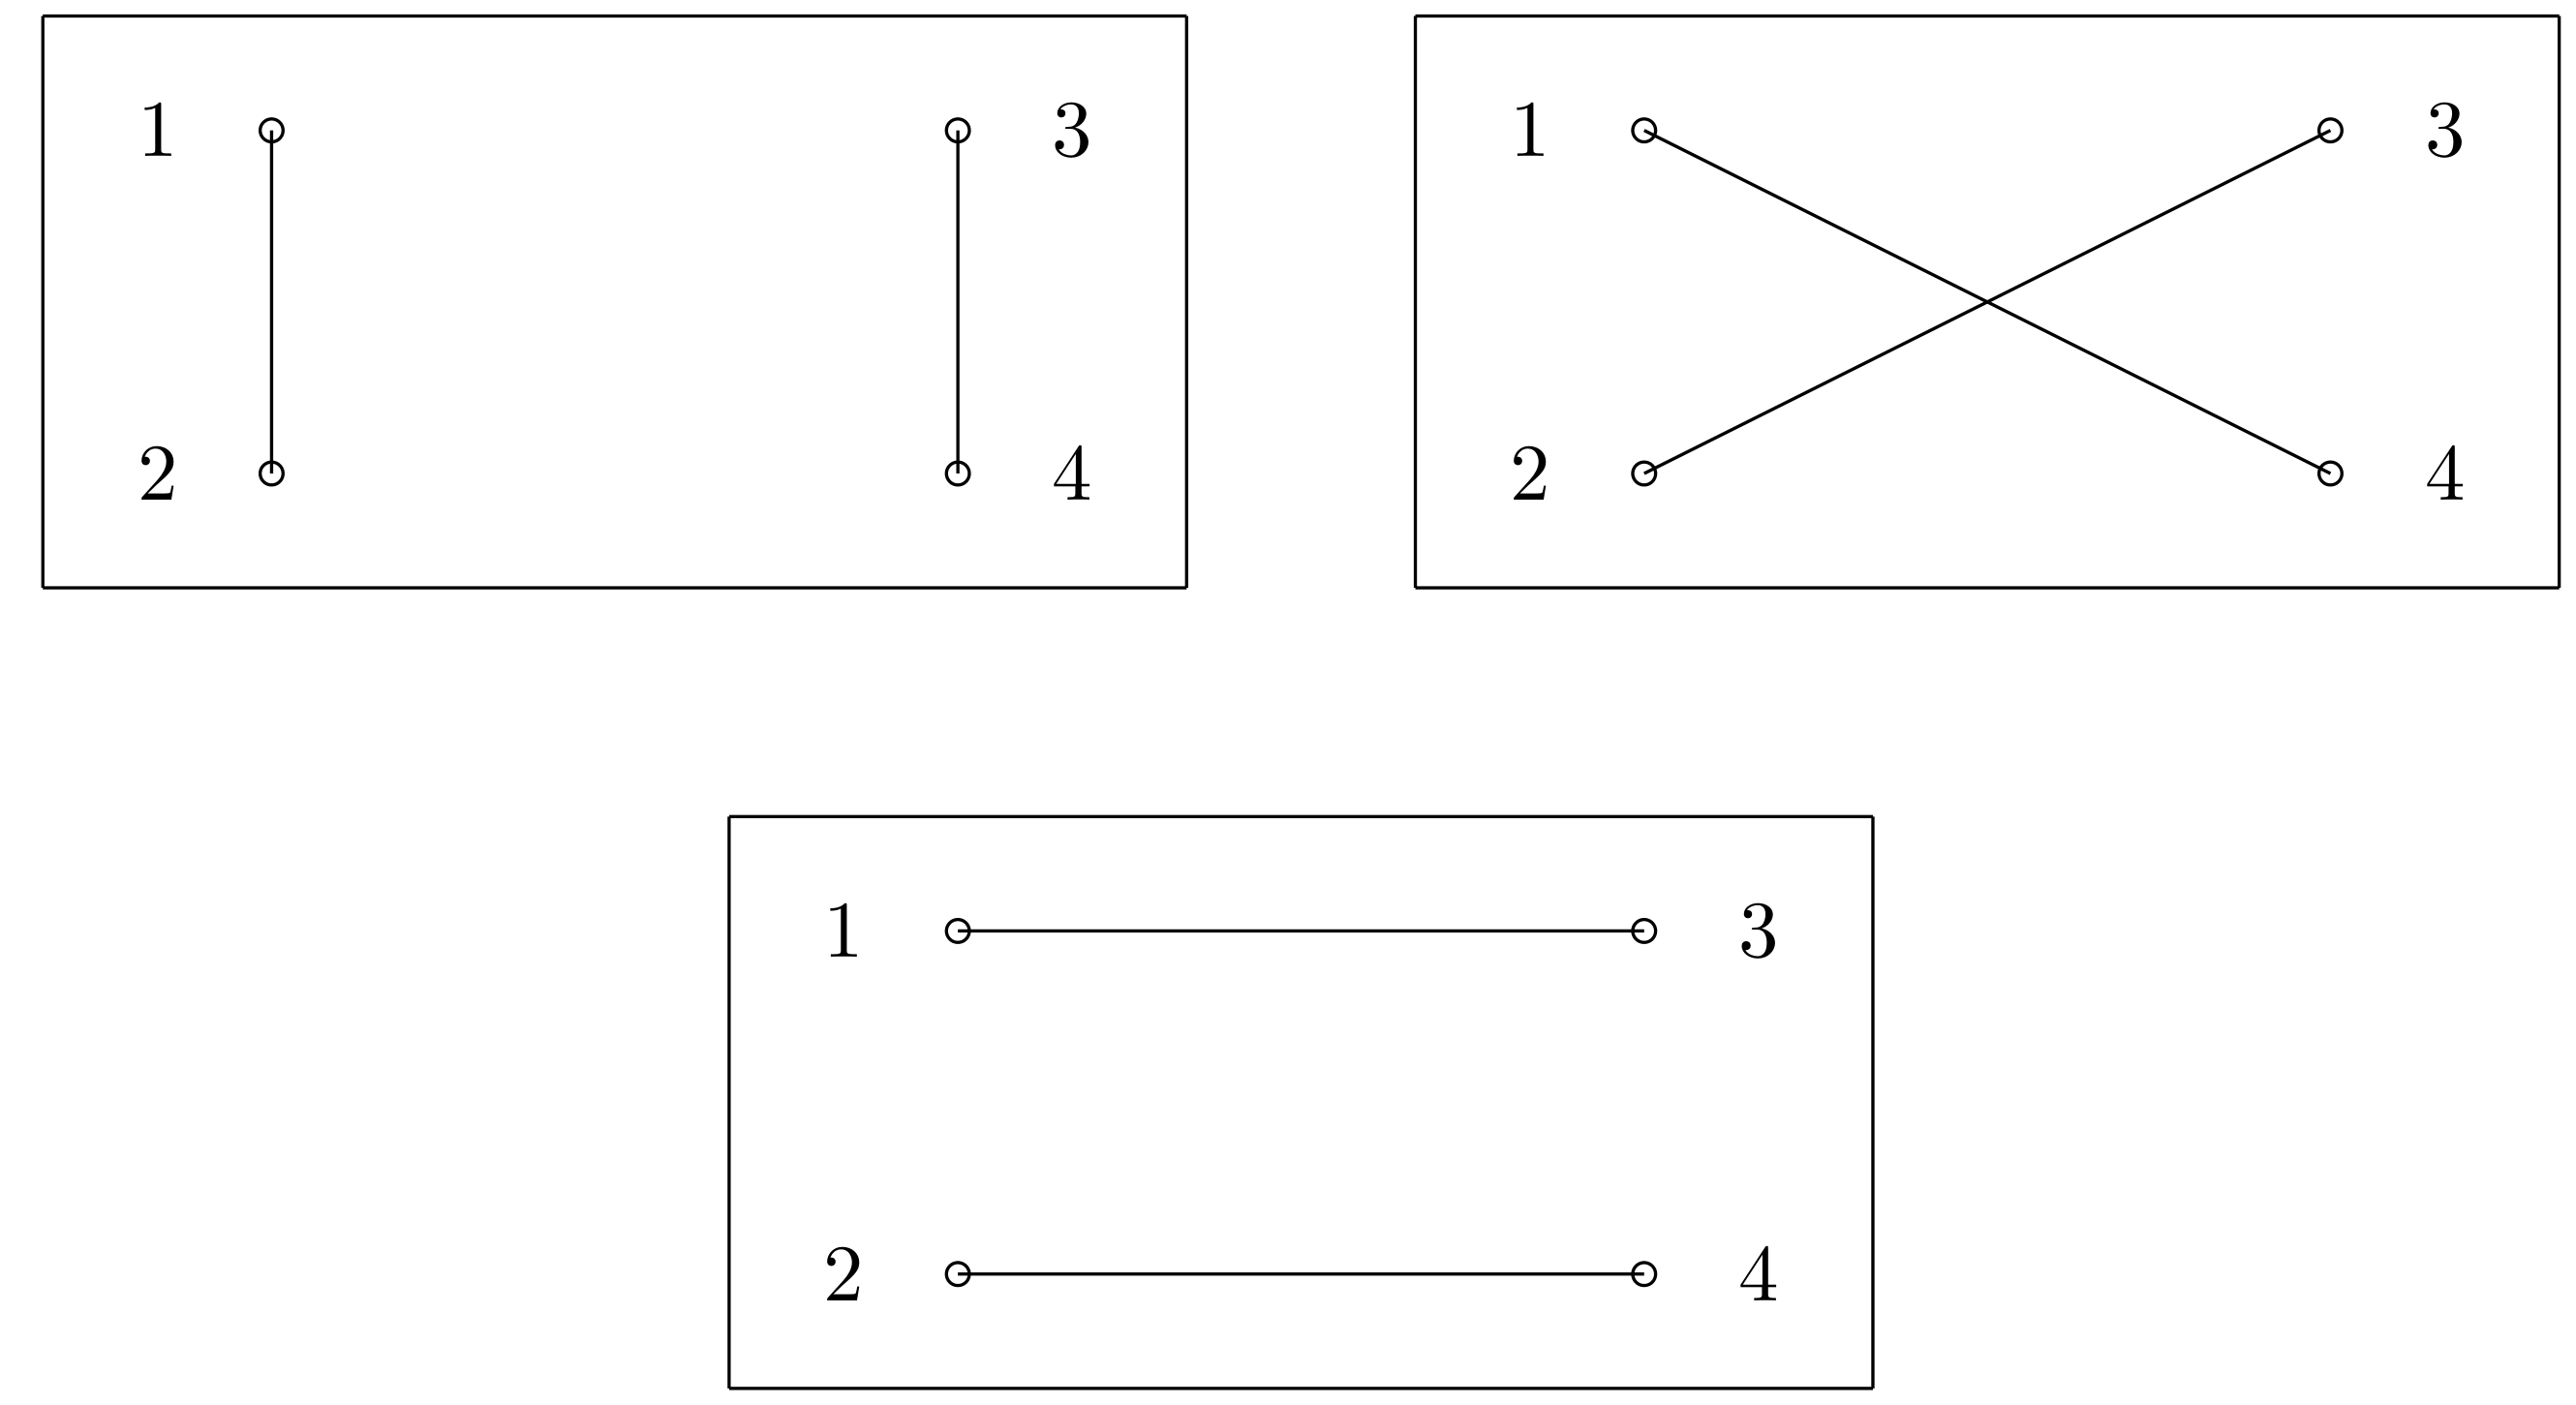
\includegraphics[width=11.26cm]{figures/fig-01.png}
  \caption{集合 $\{1, 2, 3, 4 \}$ 的配对\figorig{29}{1}}
  \label{fig:1}
\end{figure}


我们用 $\Pi(T)$ 表示集合 $T$ 上所有配对构成的集合，并把 $\Pi(\lbrace{1, \ldots ,2k\rbrace})$ 记作 $\Pi_k$。显然 $|\Pi_k|=\frac{(2k)!}{2^k\cdot k!}=(2k-1)!!$。对任意 $\sigma\in \Pi_k$，可把 $\sigma$ 看作 $\lbrace{1, \ldots ,2k\rbrace}$ 的一个置换，满足 $\sigma^2=1$ 且 $\sigma$ 没有不动点。也就是说，$\sigma$ 把任一元素 $i$ 映到含 $i$ 的那一对中的另一个元素 $\sigma(i)$。

\begin{theorem}\label{wick}（Wick 定理）设 $B^{-1}$ 表示 $B$ 在 $V^*$ 上的逆形式，$\ell_1, \ldots ,\ell_N\in V^*$。
则当 $N$ 为偶数时，有
$$
\int_{V}\ell_1(x) \ldots \ell_N(x)e^{-\frac{B(x,x)}{2}}dx=
\frac{(2\pi)^{\frac{d}{2}}}{\sqrt{\det B}}
\sum_{\sigma\in \Pi_{N/2}}\prod_{i\in \lbrace{1, \ldots ,N\rbrace}/\sigma}
B^{-1}(\ell_i,\ell_{\sigma(i)})
$$
当 $N$ 为奇数时，该积分为零。
\end{theorem}

\begin{proof} 若 $N$ 为奇数，结论显然，因为被积函数是奇函数。故考虑偶数情形 $N=2k$。
由于等式两边都是 $\ell_1, \ldots ,\ell_N$ 的对称多重线性型，
只需在 $\ell_1= \cdots =\ell_N=\ell$ 时证明结论。
此外，显然所讨论的公式在线性变量替换下不变，
因此可以选取坐标系使 $B(x,x)=x_1^2+ \cdots +x_d^2$、$\ell(x)=x_1$。
于是只需假设 $d=1$ 且 $\ell(x)=x$。
此时定理断言
$$
\int_{-\infty}^{\infty}x^{2k}e^{-\frac{x^2}{2}}dx=(2\pi)^{\frac{1}{2}}(2k-1)!!,
$$
这正是公式 \eqref{gammaint}。
\end{proof}

\begin{example} 我们有
$$
\int_{V}\ell_1(x)\ell_2(x)e^{-\frac{B(x,x)}{2}}dx=
\frac{(2\pi)^{\frac{d}{2}}}{\sqrt{\det B}}
B^{-1}(\ell_1,\ell_2),
$$
\scriptsize
$$
\int_{V}\ell_1(x)\ell_2(x)\ell_3(x)\ell_4(x)e^{-\frac{B(x,x)}{2}}dx=
$$
$$
\frac{(2\pi)^{\frac{d}{2}}}{\sqrt{\det B}}
(B^{-1}(\ell_1,\ell_2)B^{-1}(\ell_3,\ell_4)+
B^{-1}(\ell_1,\ell_3)B^{-1}(\ell_2,\ell_4)+
B^{-1}(\ell_1,\ell_4)B^{-1}(\ell_2,\ell_3)).
$$
\normalsize
\end{example}

Wick 定理表明，$a_i$ 的计算问题具有组合本性。事实上，在这一计算中起核心作用的是某些有限图，称为\emph{Feynman 图}。它们是本节余下部分的主要研究对象。

% [Tutor Note: 计数要点——$2k$ 个标记点的配对数满足 $|\Pi_k|=\frac{(2k)!}{2^k k!}=(2k-1)!!$：先对 $2k$ 个点排序（$2k!$ 种），再除以每对的顺序 $2^k$ 与各对之间的顺序 $k!$。这与高斯矩 $\int x^{2k}e^{-x^2/2}dx=(2k-1)!!\sqrt{2\pi}$ 的系数完全一致；定理证明中“令 $\ell_1=\cdots=\ell_N=\ell$ 再作正交变换把 $B$ 化为标准形”是化归到 $d=1$ 的关键，但这一步只对多重线性型成立，$g$ 为一般多项式时不能这样化归。自由理论的归一化因子 $(2\pi)^{d/2}/\sqrt{\det B}$ 恰是“无边图的真空振幅”，可用作核对后续 Feynman 规则中每个连通分量的整体系数。]

\subsection{Feynman 图与 Feynman 定理} \label{fdft}
我们回到系数 $a_i$ 的计算问题。
由于每个具体的 $a_i$ 只依赖于 $g$ 在 $c$ 处的有限阶导数，故不妨假设 $g$ 是多项式，或更具体地说，是线性函数之积：
$g=\ell_1 \ldots \ell_N$，$\ell_i\in V^*$。因此，只需能够计算积分
\begin{equation}\label{expaa}
\langle\ell_1 \ldots \ell_N\rangle:= \hbar^{-\frac{d}{2}}e^{\frac{S(c)}{\hbar}}\int_{D}
\ell_1(x) \ldots\ell_N(x)e^{-\frac{S(x)}{\hbar}}dx.
\end{equation}
的级数展开。

不失一般性，可设 $c=0$ 且 $S(c)=0$。
于是 $S$ 在 $c$ 处的（渐近）Taylor 展开为
$$
S(x)=\frac{B(x,x)}{2}-\sum_{i\ge 3}\frac{B_i(x,\ldots,x)}{i!},
$$
其中 $B_i:=d^if(0)$。因此，把 \eqref{expaa} 的左端视为 $\hbar$ 的幂级数，并作变量替换 $x\mapsto \hbar^{\frac{1}{2}}x$（与上一节相同），得到
$$
\langle\ell_1 \ldots \ell_N\rangle=
\hbar^{\frac{N}{2}}\int_V \ell_1(x) \ldots \ell_N(x)e^{-\frac{B(x,x)}{2}+
\sum_{i\ge 3}\hbar^{\frac{i}{2}-1}\frac{B_i(x, \ldots ,x)}{i!}}dx.
$$
注意，这只是在 $\hbar$ 的渐近展开意义下的等式，因为我们忽略了用全空间代替区域 $D$ 所产生的快速衰减误差。但它特别蕴涵：当 $\hbar\to 0$ 时 $\langle\ell_1 \ldots \ell_N\rangle=O(\hbar^{\lceil\frac{N}{2}\rceil})$（因为展开式中只含 $\hbar$ 的整数幂）。

下面的定理归功于 Feynman，它以 Feynman 图的形式给出该积分的值。
该定理容易证明，却是量子场论的核心，并将成为我们的主要定理之一。在陈述 Feynman 定理之前，先引入一些记号。

设 $G_{\ge 3}(N)$ 表示满足下述条件的图的同构类之集：有 $N$ 个 1 价“外”顶点，标记为 $1, \ldots ,N$；还有有限个无标记的“内”顶点，其价数任意且 $\ge 3$。注意这里及以下均允许图在两个顶点之间有多重边，也允许顶点到自身的自环（见图~\ref{fig:2}）。

\begin{figure}[htbp]
  \centering
  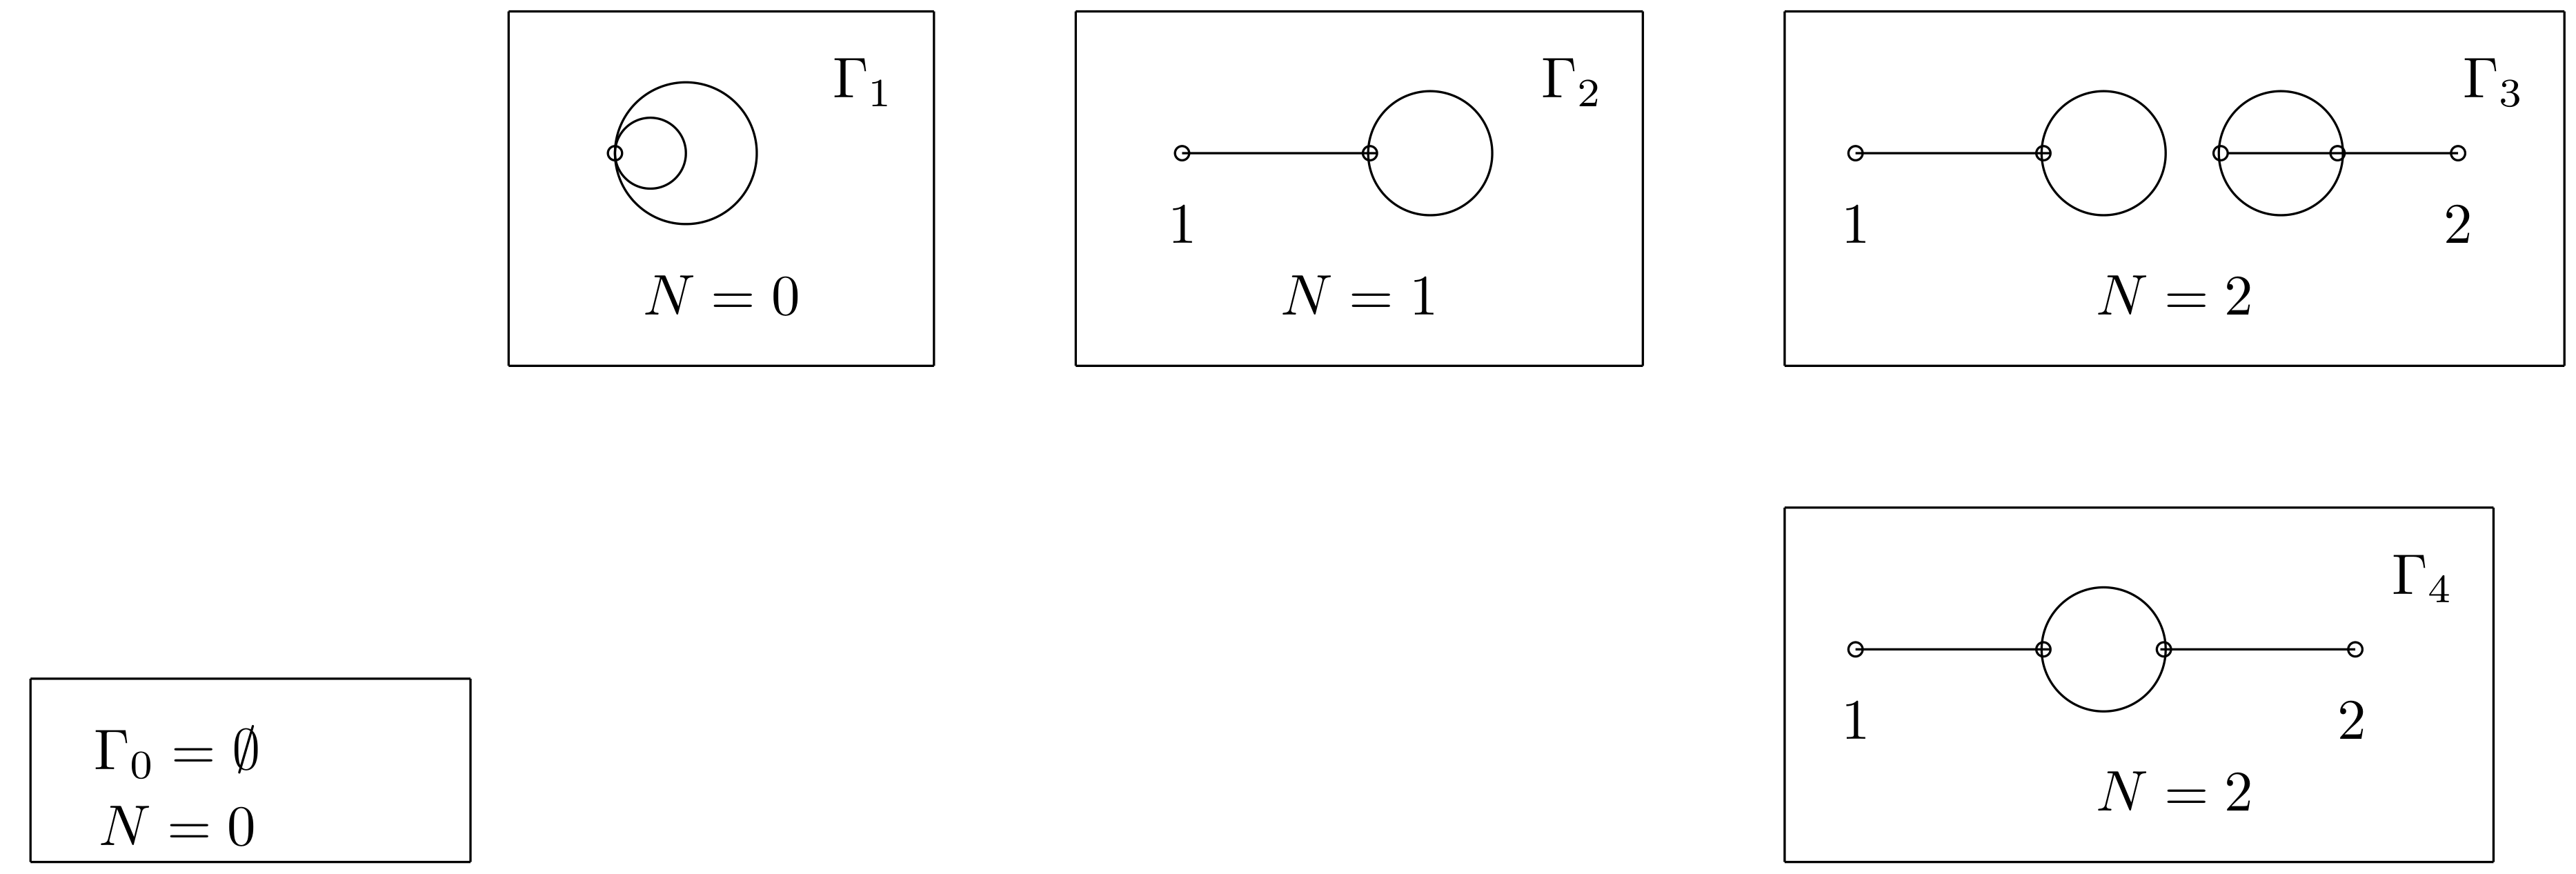
\includegraphics[width=15.6cm]{figures/fig-02.png}
  \caption{$G_{\ge 3} (N)$ 的元素示例。\figorig{31}{2}}
  \label{fig:2}
\end{figure}

对每个图 $\Gamma\in G_{\ge 3}(N)$，如下定义 $\Gamma$ 的\emph{Feynman 振幅}。

1. 把余向量 $\ell_j$ 放在第 $j$ 个外顶点上。

2. 在每个 $i$ 价内顶点上放张量 $B_i$。

3. 用双线性型 $B^{-1}$ 沿 $\Gamma$ 的边对这些张量作缩并。
由此得到一个数，称为 $\Gamma$ 的\emph{（Feynman）振幅}，记作 $F_\Gamma(\ell_1, \ldots ,\ell_N)$。

\begin{remark} 若 $\Gamma$ 不连通，则 $F_\Gamma$ 定义为各连通分量所得数之积。此外，空图的振幅定义为 $1$。
\end{remark}

\begin{example} 设
$$
B_3:=\sum_i b_i^{13}\otimes b_i^{23}\otimes b_i^{33},\ 
B_4:=\sum_j b_j^{14}\otimes b_j^{24}\otimes b_j^{34}\otimes b_j^{44},
$$
其中 $b_i^{jk}\in V^*$。则对图~\ref{fig:2} 中的图 $\Gamma_3$，其振幅等于
\scriptsize
$$
F_{\Gamma_3}(\ell_1,\ell_2)=
$$
$$
\sum_i B^{-1}(\ell_1,b_i^{13})B^{-1}(b_i^{23},b_i^{33})\cdot \sum_{i,j} B^{-1}(b_i^{13},b_j^{14})B^{-1}(b_i^{23},b_j^{24})B^{-1}(b_i^{33},b_j^{34})B^{-1}(b_j^{44},\ell_2).
$$
\normalsize
\end{example}

\begin{theorem}\label{Feyn}（Feynman）
有
\begin{equation}\label{Feynsum}
\langle\ell_1 \ldots \ell_N\rangle=
\frac{(2\pi)^{\frac{d}{2}}}{\sqrt{\det B}}
\sum_{\Gamma\in G_{\ge 3}(N)}\frac{\hbar^{b(\Gamma)}}{|{\rm Aut}(\Gamma)|}
F_\Gamma(\ell_1, \ldots ,\ell_N),
\end{equation}
其中 $b(\Gamma)$
是 $\Gamma$ 的边数减去内顶点数。
\end{theorem}
这里 ${\rm Aut}(\Gamma)$ 表示 $\Gamma$ 的自同构群；所谓 $\Gamma$ 的自同构，是指对顶点\textbf{与}边的一个置换（可以翻转自环），它固定每个外顶点并保持图的结构，见图~\ref{fig:3}。因此可能存在非平凡的自同构：有的在顶点集上作用平凡，有的甚至在边集上也作用平凡。例如，存在 $\Gamma_4$ 的一个自同构翻转上下两条弧，以及 $\Gamma_2$ 的一个自同构翻转自环。

\begin{figure}[htbp]
  \centering
  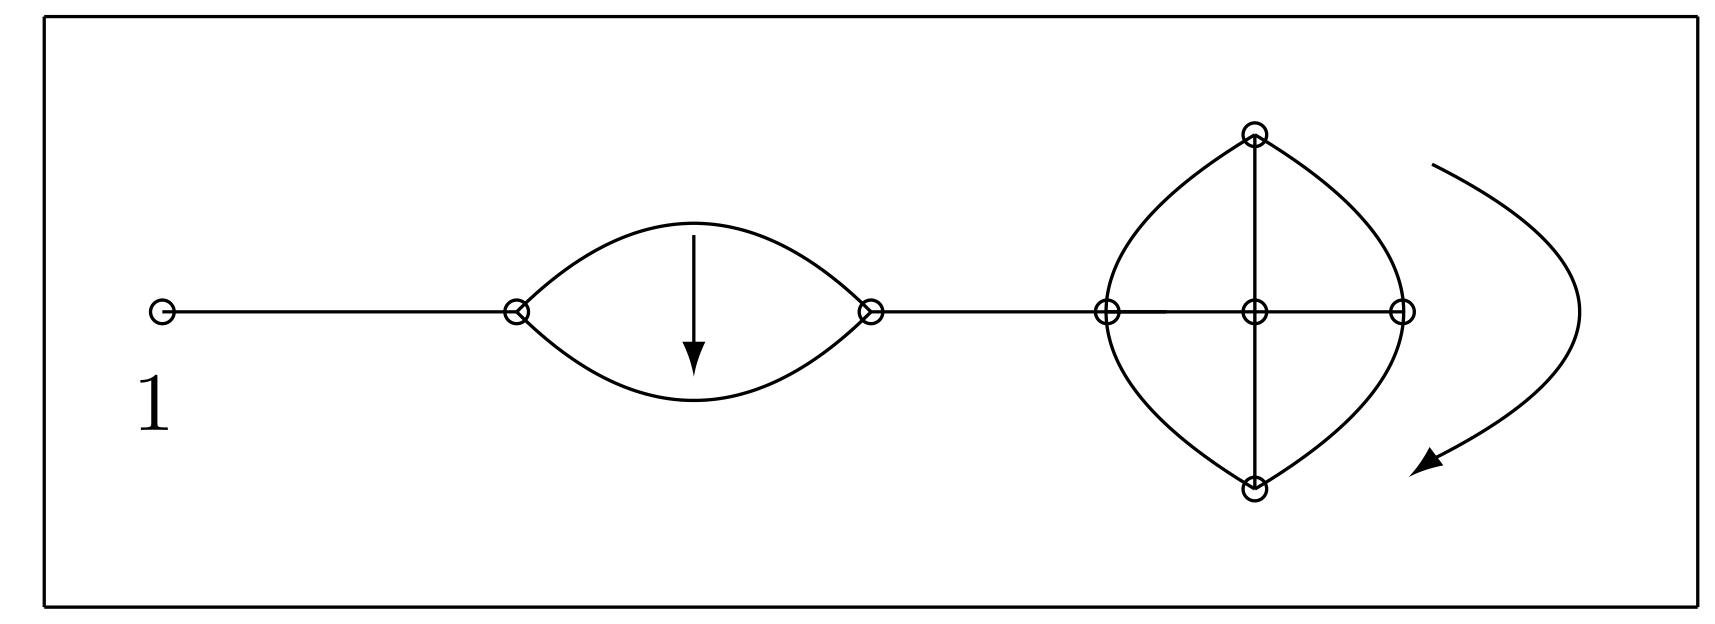
\includegraphics[width=7.26cm]{figures/fig-03.png}
  \caption{图的一个自同构\figorig{32}{3}}
  \label{fig:3}
\end{figure}


\begin{remark} 1. 注意这个和是无穷和，但按 $\hbar$ 的幂次形式收敛（形式幂级数意义下收敛）。

2. 定理 \ref{Feyn} 是 Wick 定理的推广：取 $S(x)=\frac{B(x,x)}{2}$ 即得后者。事实上，此时给出非零振幅的图没有内顶点，故归结为对应于配对 $\sigma$ 的图。
\end{remark}

现在对术语作一些说明。在量子场论中，函数 $\langle\ell_1 \ldots \ell_N\rangle$ 称为\emph{N 点关联函数}，图 $\Gamma$ 称为\emph{Feynman 图}。置于边上的型 $B^{-1}$ 称为\emph{传播子}。函数 $S$ 的展开中的三次及更高次项 $\frac{B_i}{i!}$ 称为\emph{相互作用项}，因为这类项（在作用量泛函中）描述粒子间的相互作用。$S$ 为二次型（即无相互作用）的情形称为\emph{自由理论}；也就是说，对自由理论，关联函数由 Wick 公式确定。

\begin{remark}\label{G3*} 有时考虑归一化关联函数是方便的：
$$
\langle\ell_1\ldots\ell_N\rangle_{\rm norm}:=\frac{\langle\ell_1\ldots\ell_N\rangle}{\langle\emptyset\rangle}
$$
其中 $\langle\emptyset\rangle$ 表示无插入时的积分。
Feynman 定理蕴涵它们由下述公式给出：
$$
\langle\ell_1 \ldots \ell_N\rangle_{\rm norm}=
\sum_{\Gamma\in G_{\ge 3}^*(N)}\frac{\hbar^{b(\Gamma)}}{|{\rm Aut}(\Gamma)|}
F_\Gamma(\ell_1, \ldots ,\ell_N),
$$
其中 $G^*_{\ge 3}(N)$ 是 $G_{\ge 3}(N)$ 中所有不含没有外顶点的连通分量的那些图构成的子集。
\end{remark}

% [Tutor Note: 对称因子——定理中的 $|{\rm Aut}(\Gamma)|$ 必须连同边一起计算：除顶点置换外，交换两条平行边、以及翻转自环（如原文中 $\Gamma_2$ 的自环、$\Gamma_4$ 的上下弧）都算非平凡自同构。检验办法：把图的所有半边（half-edge）视为可区分对象，$\prod_i i!^{n_i}n_i!$ 是“半边标记方式数”，除以 $|{\rm Aut}(\Gamma)|$ 才是同一图的相异标记数（轨道—稳定子定理）；对 $N$ 点函数，外顶点标记固定，故 $(2N-1)!!$ 只出现在无内顶点的 Wick 情形，一般图没有简单的双阶乘公式。]

% [Tutor Note: 原文疑误——第 2 小节中 $B_i:=d^if(0)$ 的 $f$ 应为 $S$，即 $B_i:=d^iS(0)$；由上下文 $S(x)=\frac{B(x,x)}{2}-\sum_{i\ge3}B_i(x,\ldots,x)/i!$ 亦可判定。另外术语一段 “propagator” 后原文多写了一个句点（“propagator}..”），译文按单句点处理。]

\subsection{Feynman 定理的加权版本}
在证明定理 \ref{Feyn} 之前，我们先对它略作修改与推广。即在量子场论中，常把相互作用理论视为自由理论的形变。
这意味着 $S(x)=\frac{B(x,x)}{2}+\widetilde S(x)$，其中 $\widetilde S(x)$ 是微扰
$$
\widetilde S(x):=-\sum_{i\ge 0}g_i\frac{B_i(x, \ldots ,x)}{i!}
$$
而 $g_r, r\ge 0$ 是（形式）参数。这些参数的一个好处是：它们使我们能按各价数顶点的数目，对和式 \eqref{Feynsum} 中 Feynman 图的振幅进行归并。
具体地说，把\emph{配分函数}
$$
Z=\hbar^{-\frac{d}{2}}\int_V e^{-\frac{S(x)}{\hbar}}dx
$$
视为 $g_i$ 的级数。
设 $\bold n=(n_0,n_1,n_2, \ldots )$ 是非负整数序列，其中几乎所有的项都为零。
设 $G(\bold n)$ 表示具有 $n_0$ 个 0 价顶点、$n_1$ 个 1 价顶点、$n_2$ 个 2 价顶点等的图的同构类之集
（因此，现在考虑的是无外顶点的图）。对 $\Gamma\in G(\bold n)$，以 $F_\Gamma$ 记如前定义的 $\Gamma$ 的振幅。于是
$$
F_\Gamma=\prod_i{g_i^{n_i}}\cdot \Bbb F_\Gamma, 
$$
其中 $\Bbb F_\Gamma$ 是不含因子 $g_j$ 时算得的 Feynman 振幅。

\begin{theorem}\label{Feyn1}
有
$$
Z=
\frac{(2\pi)^{\frac{d}{2}}}{\sqrt{\det B}}
\sum_{\bold n}
\sum_{\Gamma\in G(\bold n)}\frac{\hbar^{b(\Gamma)}}{|{\rm Aut}(\Gamma)|}
F_\Gamma=
$$
$$
\frac{(2\pi)^{\frac{d}{2}}}{\sqrt{\det B}}
\sum_{\bold n}\prod_i({g_i\hbar^{\frac{i}{2}-1})^{n_i}}
\sum_{\Gamma\in G(\bold n)}\frac{\Bbb F_\Gamma}{|{\rm Aut}(\Gamma)|},
$$
其中 $b(\Gamma)=\sum_i n_i(\frac{i}{2}-1)$
是 $\Gamma$ 的边数减去顶点数。
\end{theorem}

注意，可以把 $Z$ 视为代数
$$
\Bbb C[g_0\hbar^{-\frac{3}{2}},g_1\hbar^{-1},g_2\hbar^{-\frac{1}{2}}; g_j,j\ge 3][[\hbar^{\frac{1}{2}}]],
$$
的元素，亦即它可以特殊化为
$$
g_0\hbar^{-\frac{3}{2}},g_1\hbar^{-1},g_2\hbar^{-\frac{1}{2}},g_3,g_4,...,
$$
的数值，从而给出 $\Bbb C[[\hbar^{\frac{1}{2}}]]$ 中的一个元素。
此外，$Z$ 也可特殊化到 $\hbar=1$，得到 $\Bbb C[[g_j, j\ge 0]]$ 中的一个元素；而该定理实际上等价于这一特殊化。我们仍然选择保留 $\hbar$，是为了能够取经典极限 $\hbar\to 0$。

我们将在下一小节证明定理 \ref{Feyn1}。
这里先说明定理 \ref{Feyn} 实际上是定理 \ref{Feyn1} 的特例。
事实上，由于关联函数关于 $\ell_1, \ldots ,\ell_N$ 对称，只需考虑 $\ell_1= \cdots =\ell_N=\ell$ 的情形。
此时记关联函数 $\langle\ell^N\rangle$（即 $\ell^N$ 的期望值）。显然，为对所有 $N$ 计算 $\langle\ell^N\rangle$，只需计算生成函数
$$
\langle e^{\ell}\rangle=\hbar^{-\frac{d}{2}}\int_Ve^{\ell(x)-\frac{S(x)}{\hbar}}dx:=\sum_{N=0}^\infty \frac{\langle\ell^N\rangle}{N!},
$$
它在相差一个缩放因子以及把 $\ell$ 乘以 $i$ 的意义下，就是 Feynman 密度 $e^{-\frac{S(x)}{\hbar}}dx$ 的 Fourier 变换。但这个期望值恰好就是定理 \ref{Feyn1} 在 $g_i=1$（$i\ge 3$）、$g_0=g_2=0$、$g_1=\hbar $、$B_1=\ell$、$B_0=0$、$B_2=0$ 时给出的期望值。因此，定理 \ref{Feyn1} 蕴涵定理 \ref{Feyn}（分母中的因子 $N!$ 可由下述事实解释：定理 \ref{Feyn1} 中考虑的是无标记的 1 价顶点，而不是有标记的）。

\subsection{Feynman 定理的证明}
现在证明定理 \ref{Feyn1}。
作变量替换 $y=\hbar^{-\frac{1}{2}}x$。
把指数函数展开为 Taylor 级数，得
$$
Z=\sum_{\bold n}Z_\bold n, 
$$
其中
$$
Z_\bold n=\int_V e^{-\frac{B(y,y)}{2}}
\prod_i \frac{g_i^{n_i}}{i!^{n_i}n_i!}
(\hbar^{\frac{i}{2}-1}B_i(y, \ldots ,y))^{n_i}dy.
$$
把 $B_i$ 写成线性函数之积的和，并利用 Wick 定理可知，对每个 $\bold n$，该积分的值可以如下组合地表达。

1. 对每个因子 $B_i$ 配一朵“花”——一个带 $i$ 条出边的顶点（见图~\ref{fig:4}）。

\begin{figure}[htbp]
  \centering
  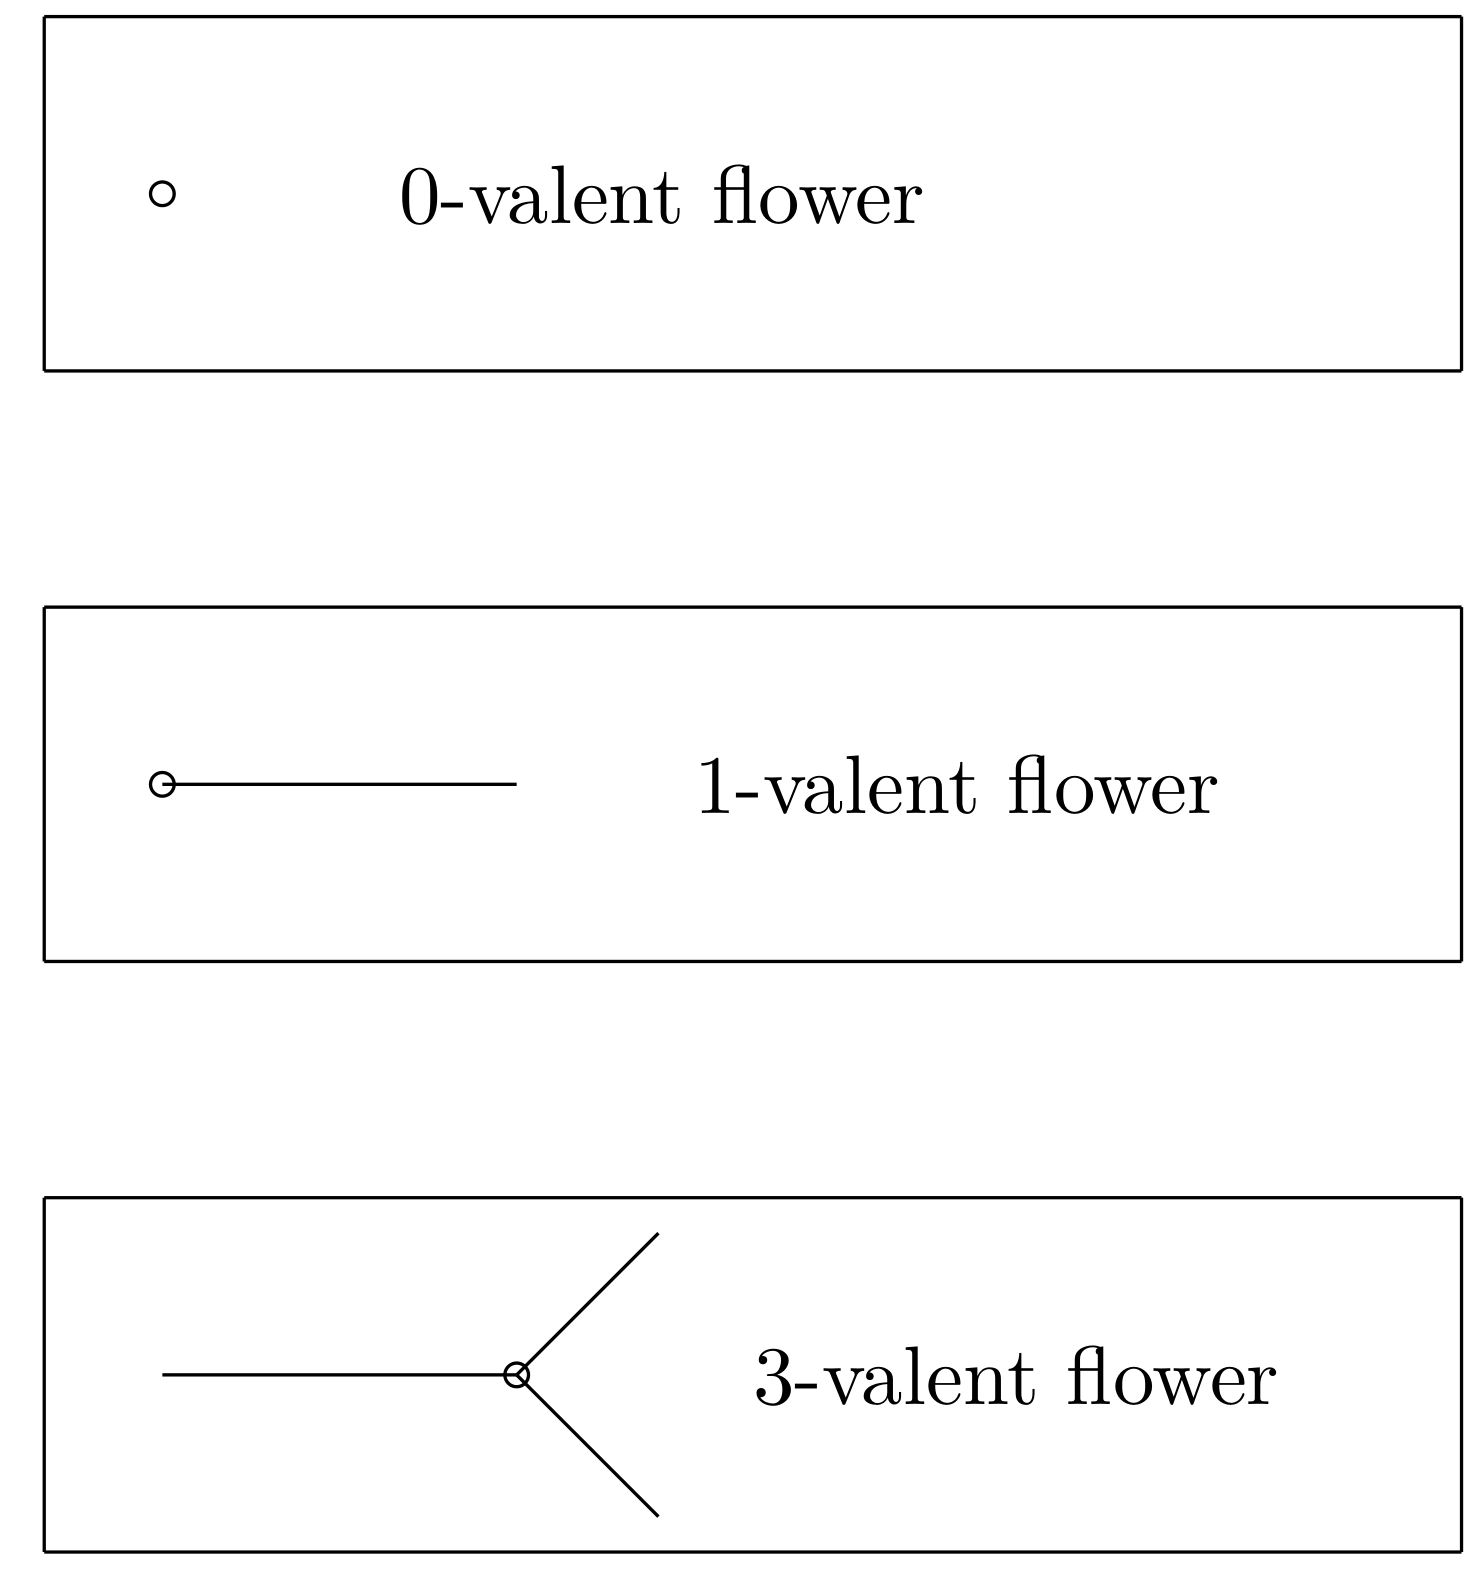
\includegraphics[width=6.26cm]{figures/fig-04.png}
  \caption{（原文无图题）\figorig{35}{4}}
  \label{fig:4}
\end{figure}


2. 考虑这些出边的端点构成的集合 $T_{\bold n}$（见图~\ref{fig:5}），并对该集合的任一配对 $\sigma$，考虑用型 $B^{-1}$ 对张量 $B_i$ 所作的相应缩并。由此得到标量 $\Bbb F(\sigma)$。

\begin{figure}[htbp]
  \centering
  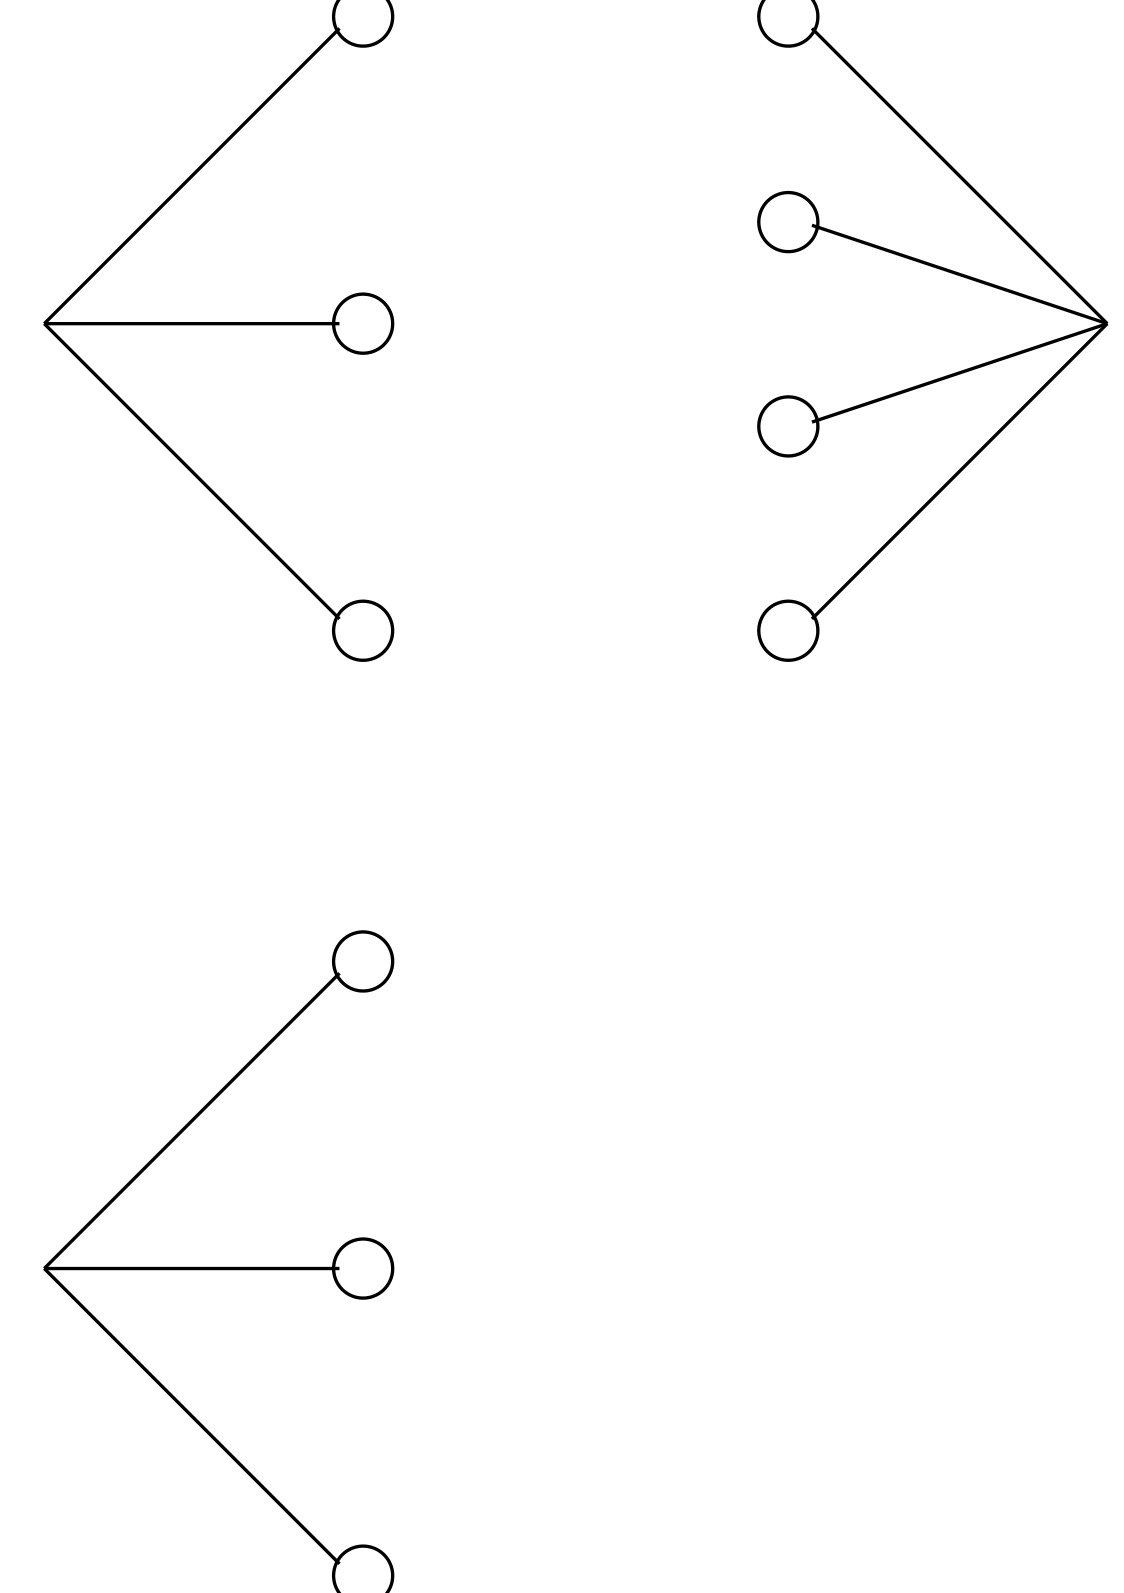
\includegraphics[width=4.76cm]{figures/fig-05.png}
  \caption{$\bold n = (0, 0, 0, 2, 1, 0, 0,       \ldots)$ 时的集合 $T_\bold n$（白色圆圈构成的集合）\figorig{35}{5}}
  \label{fig:5}
\end{figure}


3. 积分 $Z_{\bold n}$ 由下式给出：
\begin{equation}\label{sumpair}
Z_{\bold n}=\frac{(2\pi)^{\frac{d}{2}}}{\sqrt{\det B}}\prod_i
\frac{g_i^{n_i}}{i!^{n_i}n_i!}\hbar^{n_i(\frac{i}{2}-1)} \sum_{\sigma\in \Pi(T_{\bold n}) }\Bbb F(\sigma).
\end{equation}

现在回忆，集合上的配对可以这样可视化：把集合的元素画成点，并用边把它们连接起来。若对集合 $T_{\bold n}$ 这样做，则所有出边的端点都将以某种方式彼此连接，亦即得到一个（无向）图 $\Gamma=\Gamma_\sigma$（见图~\ref{fig:6}）。此外，容易看出标量 $\Bbb  F(\sigma)$ 正是振幅 $\Bbb F_\Gamma$。

\begin{figure}[htbp]
  \centering
  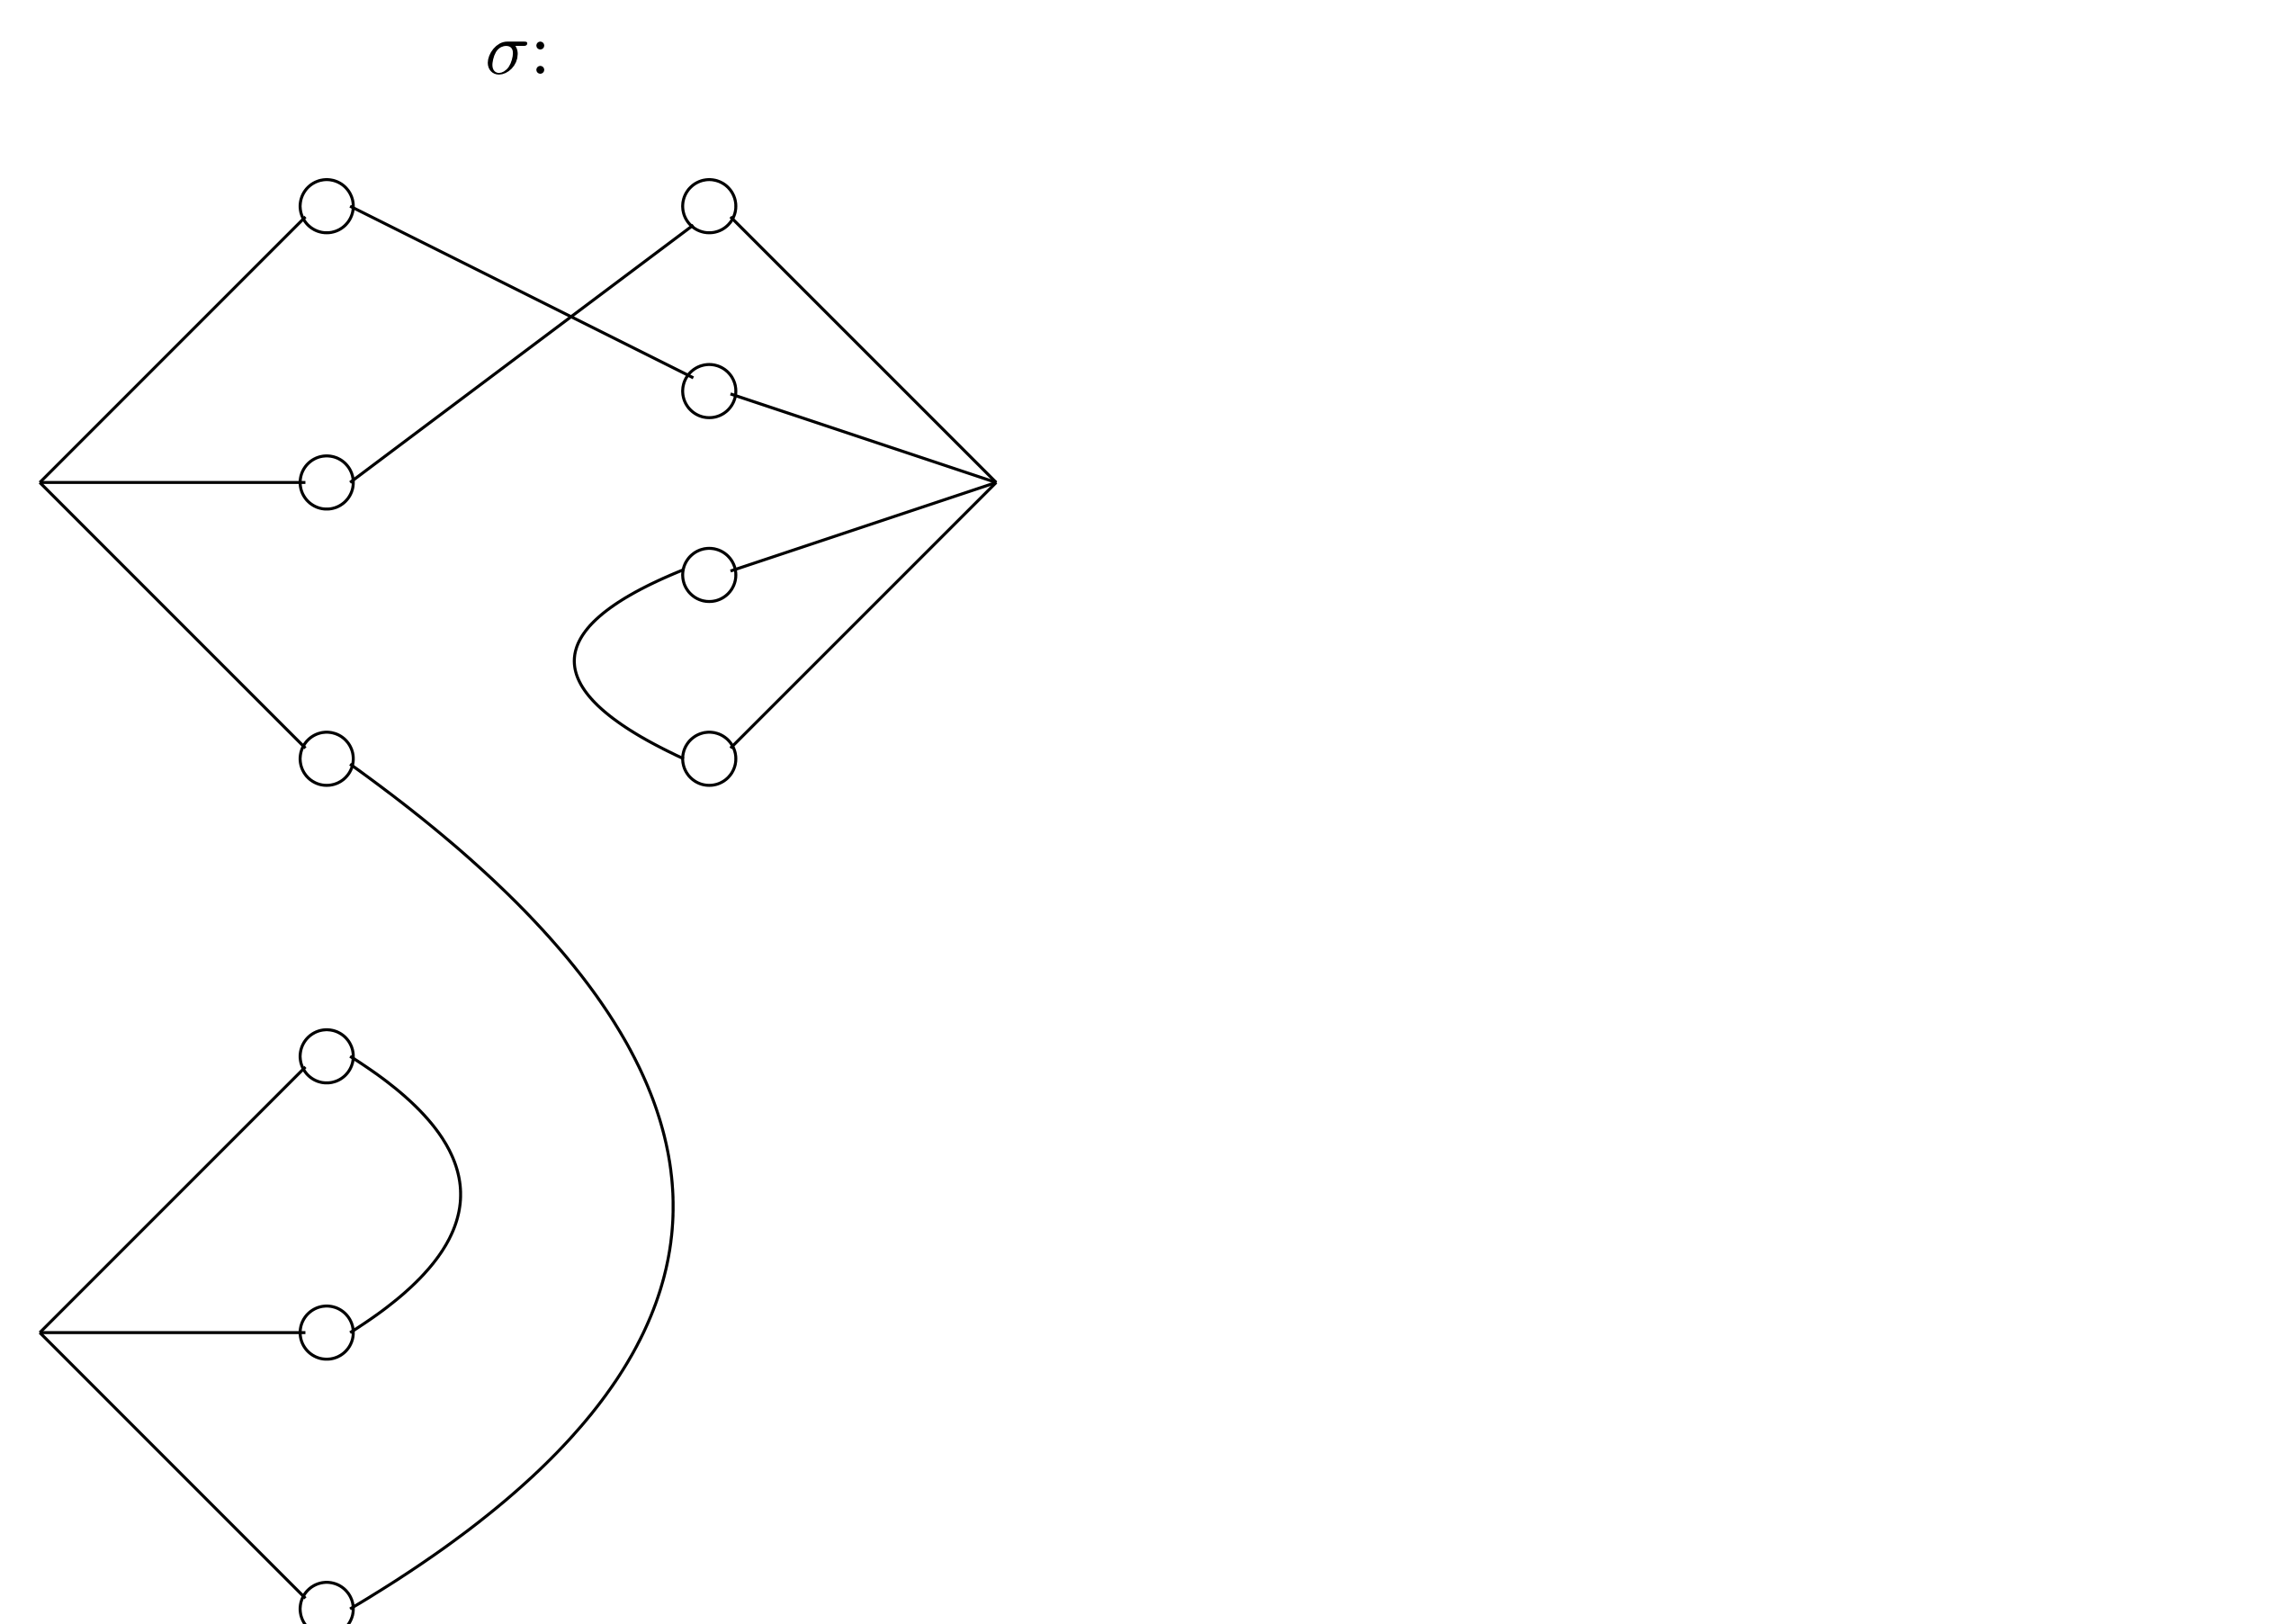
\includegraphics[width=10.76cm]{figures/fig-06.png}
  \caption{$T_{\bold n}$ 的一个配对 $\sigma$ 及相应的图 $\Gamma$。\figorig{36}{6}}
  \label{fig:6}
\end{figure}


显然，任一满足对每个 $i$ 有 $n_i$ 个 $i$ 价顶点的图 $\Gamma$ 都可由这种方式得到。然而同一个图可以以许多不同方式得到；因此，若想把对 $\sigma$ 求和中的相同项归并起来，并把它变成对 $\Gamma$ 的求和，就必须求出给出给定 $\Gamma$ 的 $\sigma$ 的数目。

为此，考虑 $T_{\bold n}$ 的保持“花”的置换群 $\Bbb G_{\bold n}$（即：从同一朵花出发的任意两条边的端点，经置换后仍落在同一朵花中）。该群包含：

1) 具有给定价数的各“花”之间的置换；

2) 每朵 $i$ 价“花”内部 $i$ 条边的置换。

更确切地说，群 $\Bbb G_{\bold n}$ 是对称群的半直积
$$
\Bbb G_{\bold n}=\prod_i (S_{n_i}\ltimes S_i^{n_i}).
$$
注意 $|\Bbb G_{\bold n}|=\prod_i i!^{n_i}n_i!$，它正是公式 (\ref{sumpair}) 分母中各数之积。

群 $\Bbb G_{\bold n}$ 作用在 $T_{\bold n}$ 的全部配对 $\sigma$ 构成的集合 $\Pi(T_{\bold n})$ 上。此外，它在给出给定图 $\Gamma$ 的 $T_{\bold n}$ 的配对构成的集合 $\Pi_\Gamma(T_{\bold n})$ 上传递地作用。进而容易看出，给定配对的稳定子就是 ${\rm Aut}(\Gamma)$。因此，给出 $\Gamma$ 的配对数等于
$$
N_\Gamma=\frac{\prod_i i!^{n_i}n_i!}{|{\rm Aut}(\Gamma)|}.
$$
于是
$$
\sum_{\sigma\in \Pi(T_{\bold n})} \Bbb F(\sigma)=\sum_\Gamma \frac{\prod_i i!^{n_i}n_i!}{|{\rm Aut}(\Gamma)|}
\Bbb F_\Gamma.
$$
最后注意，方程 (\ref{sumpair}) 中 $\hbar$ 的指数为 $\sum_in_i(\frac{i}{2}-1)$，它等于 $\Gamma$ 的边数减去顶点数，亦即 $b(\Gamma)$。
把它代入 (\ref{sumpair})，即得结论。

\begin{example}\label{treeexa} 取 $d=1$、$V=\Bbb R$、$g_i=g$、对所有 $i\ge 0$ 有 $B_i=z^i$（其中 $z$ 是形式变量）、$\hbar=1$。
于是得到渐近展开
$$
\frac{1}{\sqrt{2\pi}}\int_{-\infty}^\infty e^{-\frac{x^2}{2}+ge^{zx}}=
\sum_{n\ge 0}g^n\sum_{\Gamma\in G(n,k)}\frac{z^{2k}}{|{\rm Aut}(\Gamma)|},
$$
其中 $G(n,k)$ 是 $n$ 个顶点、$k$ 条边的图的同构类之集。\footnote{该积分在 $g<0$、$z\in \Bbb R$ 时收敛，但这在这里并不重要，因为我们只是形式地考虑该积分。}
展开左端，得
$$
\sum_k\sum_{\Gamma\in G(n,k)}\frac{z^{2k}}{|{\rm Aut}(\Gamma)|}=\frac{e^{\frac{z^2n^2}{2}}}{n!},
$$
从而
$$
\sum_{\Gamma\in G(n,k)}\frac{1}{|{\rm Aut}(\Gamma)|}=\frac{n^{2k}}{2^kk!n!}.
$$
\end{example}

\begin{exercise} 用直接组合计数验证之。
\end{exercise}

% [Tutor Note: 连通性取对数（指数公式）——定理 \ref{Feyn2} 的证明本质上是说：设 $Z/Z_0=\sum_\Gamma w_\Gamma$，其中 $w_\Gamma=\hbar^{b(\Gamma)}\Bbb F_\Gamma/|{\rm Aut}(\Gamma)|$ 按连通分量乘性分解。任一图可唯一写成连通图的 $k_j$ 重不交并 $\Gamma_1^{k_1}\ldots\Gamma_l^{k_l}$，故 $\sum_\Gamma w_\Gamma=\prod_j\sum_{k_j\ge0}w_{\Gamma_j}^{k_j}/k_j!=\exp\bigl(\sum_{\Gamma\ \text{连通}}w_\Gamma\bigr)$；其中 $1/k_j!$ 来自 $k_j$ 个同构副本之间的置换对称性，恰与自同构群阶中的 $k_j!$ 因子相消。这正是配分函数的连通图（团簇）展开，物理上即“自由能/连通关联取对数”。注意归一化 $Z/Z_0$ 已把空图振幅 $1$ 除掉，故 $\log$ 展开中没有整体常数项。]

\subsection{连通图求和}
下面将说明，配分函数 $Z$ 的对数同样由对图的求和给出，但只计入连通图。这大大简化了微扰论最初几阶中对 $Z$ 的分析，因为在给定顶点数与边数时，连通图的数目远小于全部图的数目。
\begin{theorem}\label{Feyn2} 设 $Z_0=\frac{(2\pi)^{\frac{d}{2}}}{\sqrt{\det B}}$。则有
$$
\log\frac{Z}{Z_0}=\sum_{\bold n}
\prod_i(g_i\hbar^{\frac{i}{2}-1})^{n_i}
\sum_{\Gamma\in G_c(\bold n)}\frac{\Bbb F_\Gamma}{|{\rm Aut}(\Gamma)|}
$$
其中 $G_c(\bold n)$ 是 $G(\bold n)$ 中连通图之集。\footnote{我们把连通图定义为恰有一个连通分量的图。因此，空图（连通分量数为零）不视为连通图。}
\end{theorem}

\begin{proof}
  对任意图 $\Gamma_1$、$\Gamma_2$，用 $\Gamma_1\Gamma_2$ 表示 $\Gamma_1$ 与 $\Gamma_2$ 的不交并；
  对任意图 $\Gamma$，用 $\Gamma^n$ 表示 $n$ 个 $\Gamma$ 的不交并。于是每个图都可唯一地
  写成 $\Gamma_1^{k_1} \ldots \Gamma_l^{k_l}$，其中 $\Gamma_j$
  是互不同构的连通图。此外，显然有
  $\Bbb F_{\Gamma_1\Gamma_2}=\Bbb F_{\Gamma_1}\Bbb F_{\Gamma_2}$、
  $b(\Gamma_1\Gamma_2)=b(\Gamma_1)+b(\Gamma_2)$，且
  $$
  |{\rm
    Aut}(\Gamma_1^{k_1} \ldots \Gamma_l^{k_l})|= \prod_j|{\rm
    Aut}(\Gamma_j)|^{k_j}k_j!.
    $$
    因此，把定理 \ref{Feyn2} 的等式取指数，并利用上述事实与函数 $e^x$ 的 Taylor 级数，
  即得定理 \ref{Feyn1}。既然定理 \ref{Feyn1} 已经证明，定理 \ref{Feyn2} 也就得证。
\end{proof}

\subsection{圈展开}
注意，由于定理 \ref{Feyn2} 中的求和是对连通 Feynman 图进行的，数 $b(\Gamma)$ 等于 $\Gamma$ 中的圈数减 1。特别地，$\hbar$ 的最低次项是 $\hbar^{-1}$ 项，它是对所有树的求和；次一项是 $\hbar^0$ 项，它是对所有含一个圈（回路）的图的求和；再下一项是 $\hbar$ 项，它是对双圈图的求和，依此类推。因此，物理学家把定理 \ref{Feyn2} 的展开称为\emph{圈展开}。

我们来研究这个展开中（关于 $\hbar$）最奇异的两项，即由树与单圈图求和给出的项。

设 $x_0$ 是函数 $S$ 的临界点。由于 $g_i$ 被假定为形式参数，它存在且唯一。
设 $G^{(j)}(\bold n)$ 表示 $G_c(\bold n)$ 中具有 $j$ 个圈的图的类之集。
令
$$
\left(\log\frac{Z}{Z_0}\right)_j:=
\sum_{\bold n}\prod_ig_i^{n_i}
\sum_{\Gamma\in G^{(j)}(\bold n)}\frac{\Bbb F_\Gamma}{|{\rm Aut}(\Gamma)|},
$$
于是
$$
\log\frac{Z}{Z_0}=\sum_{j=0}^\infty \left(\log\frac{Z}{Z_0}\right)_j \hbar^{j-1}.
$$

\begin{theorem}\label{trees1l}
\begin{equation}\label{treeeq}
\left(\log\frac{Z}{Z_0}\right)_0=-S(x_0),
\end{equation}
以及
\begin{equation}\label{1loopeq}
\left(\log\frac{Z}{Z_0}\right)_1=\frac{1}{2}\log \frac{\det B}{\det S''(x_0)}.
\end{equation}
\end{theorem}

\begin{proof}
首先注意，该命题纯属组合。
特别地，这意味着只需验证：当 $S$ 是实系数多项式、形如 $\frac{B(x,x)}{2}-\sum_{i=0}^Ng_i\frac{B_i(x, \ldots,x)}{i!}$ 且 $\hbar>0$ 时，命题给出的正是方程 (\ref{treeeq})、(\ref{1loopeq}) 右端的正确渐近展开。为此，令 $Z:=\hbar^{-\frac{d}{2}}\int_{\bold B}e^{-\frac{S(x)}{\hbar}}dx$，
其中 $\bold B$ 是以 $0$ 为心的球。
对充分小的 $g_i$，函数 $S$ 在 $\bold B$ 中有唯一的全局极小点 $x_0$，且该极小点非退化。
于是由最速下降公式，有
$$
\frac{Z}{Z_0}=e^{-\frac{S(x_0)}{\hbar}}I(\hbar), 
$$
其中 $I(\hbar)\sim\sqrt{\frac{\det B}{\det
    S''(x_0)}}(1+a_1\hbar+a_2\hbar^2+ \cdots )$（渐近地）。因此，
$$
\log\frac{Z}{Z_0}=-S(x_0)\hbar^{-1}+\frac{1}{2}\log
\frac{\det B}{\det S''(x_0)}+O(\hbar).
$$
这就蕴涵了结论。
\end{proof}

% [Tutor Note: 圈展开的幂次核对——对连通图，$V-E=1-L$（$L$ 为独立圈数），故 $b(\Gamma)=E-V=L-1$。逐顶点清点亦得同一结果：每个 $i$ 价顶点贡献 $\hbar^{i/2-1}$（来自 $x\mapsto\hbar^{1/2}y$ 的 $\hbar^{i/2}$ 乘以作用量中的 $\hbar^{-1}$），每条边（传播子 $B^{-1}$）贡献 $\hbar^0$，故总和为 $\sum_i n_i(\frac{i}{2}-1)=E-V$。树图 $L=0$ 给出 $\hbar^{-1}$ 的经典项 $-S(x_0)$，单圈给出 $\hbar^0$ 的 $\frac12\log\frac{\det B}{\det S''(x_0)}$，恰与第 2 章最速下降公式的指数前因子 $I(\hbar)\sim\sqrt{\det B/\det S''(x_0)}\,(1+O(\hbar))$ 逐项吻合，可作为检验译文与公式的独立手段。]

物理学家把表达式 $(\log\frac{Z}{Z_0})_0$ 称为对量子力学量 $\hbar\log\frac{Z}{Z_0}$ 的\emph{经典（或树）近似}，而把和 $(\log\frac{Z}{Z_0})_0+\hbar(\log\frac{Z}{Z_0})_1$ 称为\emph{单圈近似}。更高阶的圈近似可类似定义。注意，经典近似是通过求出经典作用量 $S(x)$ 的临界点与临界值而得到的；在经典力学与场论的情形，这对应于求解经典运动方程。

\bigskip
\noindent\rule{\textwidth}{0.6pt}
% [Tutor Note: 本章小结——Wick 定理是自由理论的全部内容：所有关联函数由 $(2k-1)!!$ 种两两缩并给出，$d=1$ 化归把一般正定二次型的情形归结为一维高斯矩。相互作用由 $\hbar^{i/2-1}$ 的顶点引入，Feynman 定理把关联函数写成对图的求和并配有对称因子 $1/|{\rm Aut}(\Gamma)|$；取对数后只剩连通图，$\hbar$ 的幂次直接数圈数。另注原文疑误：例 \ref{treeexa} 第一个渐近展开式右端为 $\sum_{n\ge0}g^n\sum_{\Gamma\in G(n,k)}z^{2k}/|{\rm Aut}(\Gamma)|$，其中 $k$ 未被求和（应由 $\sum_k$ 或 $G(n)$ 说明）；第二个式子按 $k$ 分组，可反推原意应为双层求和，译文照录原文。]

